\section{Kinetic Theory of Ideal Gases, and Equipartition of Energy}

\instructornote{%
By Matt, Spring 2020.  Time: 30 minutes.

This lab was written as a substitute for the regular ``Kinetic Theory of Ideal Gases'' lab during the spring of 2020, when we did everything by remote instruction due to the coronavirus pandemic.  I didn't want students to attempt installing the old Atoms In Motion software on their laptops; I'm not even sure if it's theoretically possible on Apple machines.  

Activities 2 and 3 in this lab mostly keeps the structure of deriving a relationship between $P$, $V$, and $\left<  E_{\rm kin} \right>$, starting with a single atom in an $\ell \times \ell \times \ell$ box.  This lab adds a new third activity, which introduces the equipartition theorem and derives the ideal gas law.

I used this once in Spring 2020, and it went smoothly.
}

\makelabheader %(Space for student name, etc., defined in master.tex)

\medskip

%\textbf{Objectives} 


\textbf{Activity 1: An Atom in a Box}

Think of a balloon filled with helium, or a space station filled with air to breathe.  In each case, the gas molecules within the container are in constant motion, frequently colliding with the container walls.  These many microscopic collisions cause a macroscopic pressure $P$ against the walls---that's what causes the balloon to remain expanded, for instance.  In this activity, we'll take a careful look at that pressure starting with the simplest system we can imagine: a single, \textit{lonely} atom rattling back and forth inside of a box.

\medskip
\begin{enumerate}[labparts]

\begin{minipage}{0.7\textwidth}

\item Suppose an atom collides elastically against a wall as shown, bouncing off with the same speed as its initial speed $v$.  Do the $y$ and $z$ components of its velocity change?
\answerspace{0.3in}

\item What happens to the $x$ component of its velocity, $v_x$?
\answerspace{0.3in}

\end{minipage}
\begin{minipage}{0.29\textwidth}
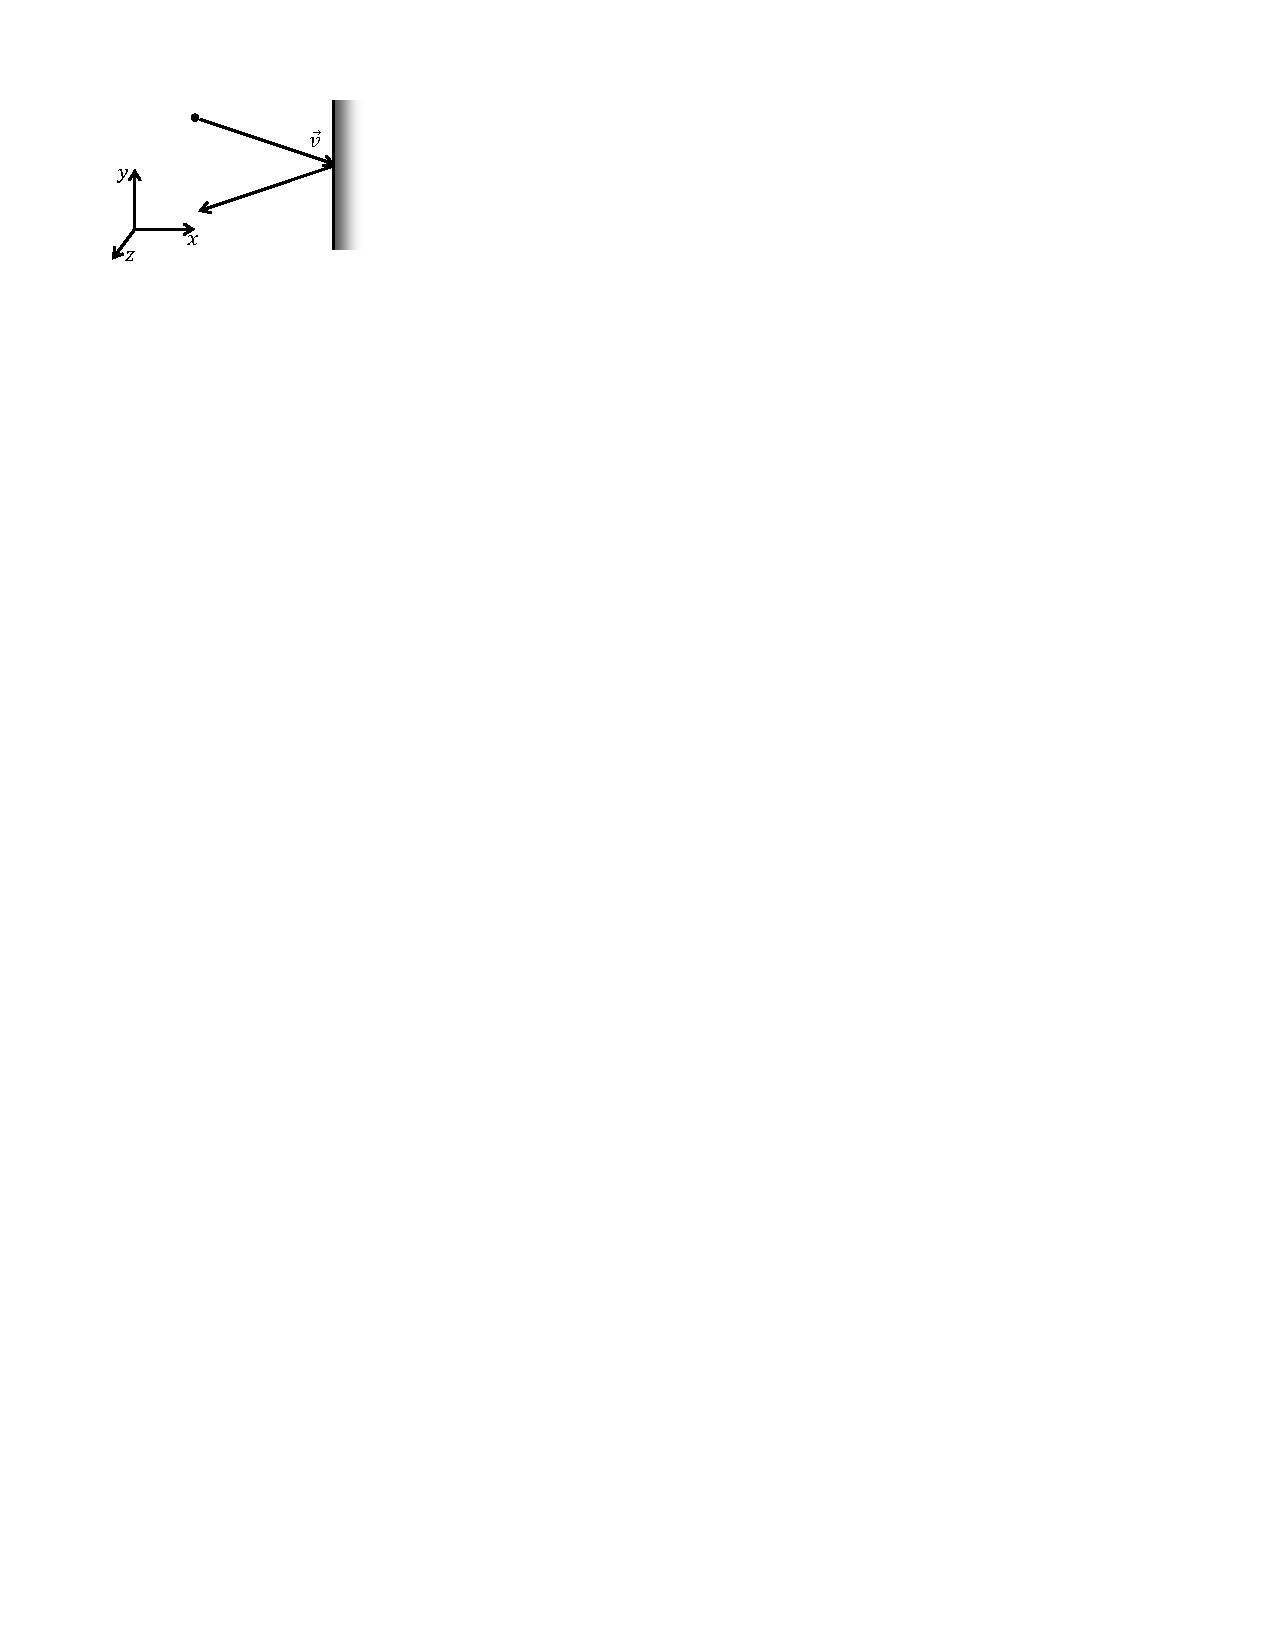
\includegraphics[width=\textwidth]{kin_theory_ideal/wall_collision.pdf}
\end{minipage}

\item Write the change in the momentum of the atom, $\Delta p = p_f - p_i$ in terms of the particle's mass $m$ and its initial $v_x$. Be careful with your signs! (Note: lower case ``$p$'' means momentum; upper case ``$P$'' means pressure.)  
\answerspace{0.3in}


\item The impulse-momentum theorem tells us that the force on the particle and its change in momentum are related by $\displaystyle \int_{t_i}^{t_f} F\,dt = \Delta p$.  We also know that we can write the average force on a particle as 
\vspace{-0.2in}
$$\displaystyle F_{\rm avg} = \dfrac{\displaystyle \int_{t_i}^{t_f} F \, dt }{ \Delta t}.$$
Use these two facts to write the average force $F_{\rm avg}$ on the atom over the time of the collision $\Delta t$ in terms of $m$, $v_x$, and $\Delta t$.
\answerspace{0.3in}

So imagine this little atom bouncing back and forth against the left and right walls of the container.  Each time it hits the right-hand wall, there's a little force of the wall on the atom, and an equal and opposite force of the atom on the wall.  To find the pressure on the wall, we really care about the \textit{average} force on the wall, over a much longer time---specifically, the time that it takes the atom to make the round trip out and back again.

\begin{minipage}{0.8\textwidth}

\item Suppose our one lonely atom is in a cubic box of dimensions $\ell \times \ell \times \ell$.  What time $\Delta t$ does it take our atom (at $v_x$) to make the round trip back and forth across the box?
\answerspace{0.3in}

\item Write the average force of the particle on the wall $F_{\rm avg}$ in terms of $m$, $v_x$ and $\ell$.
\answerspace{0.4in}

\end{minipage}
\begin{minipage}{0.19\textwidth}
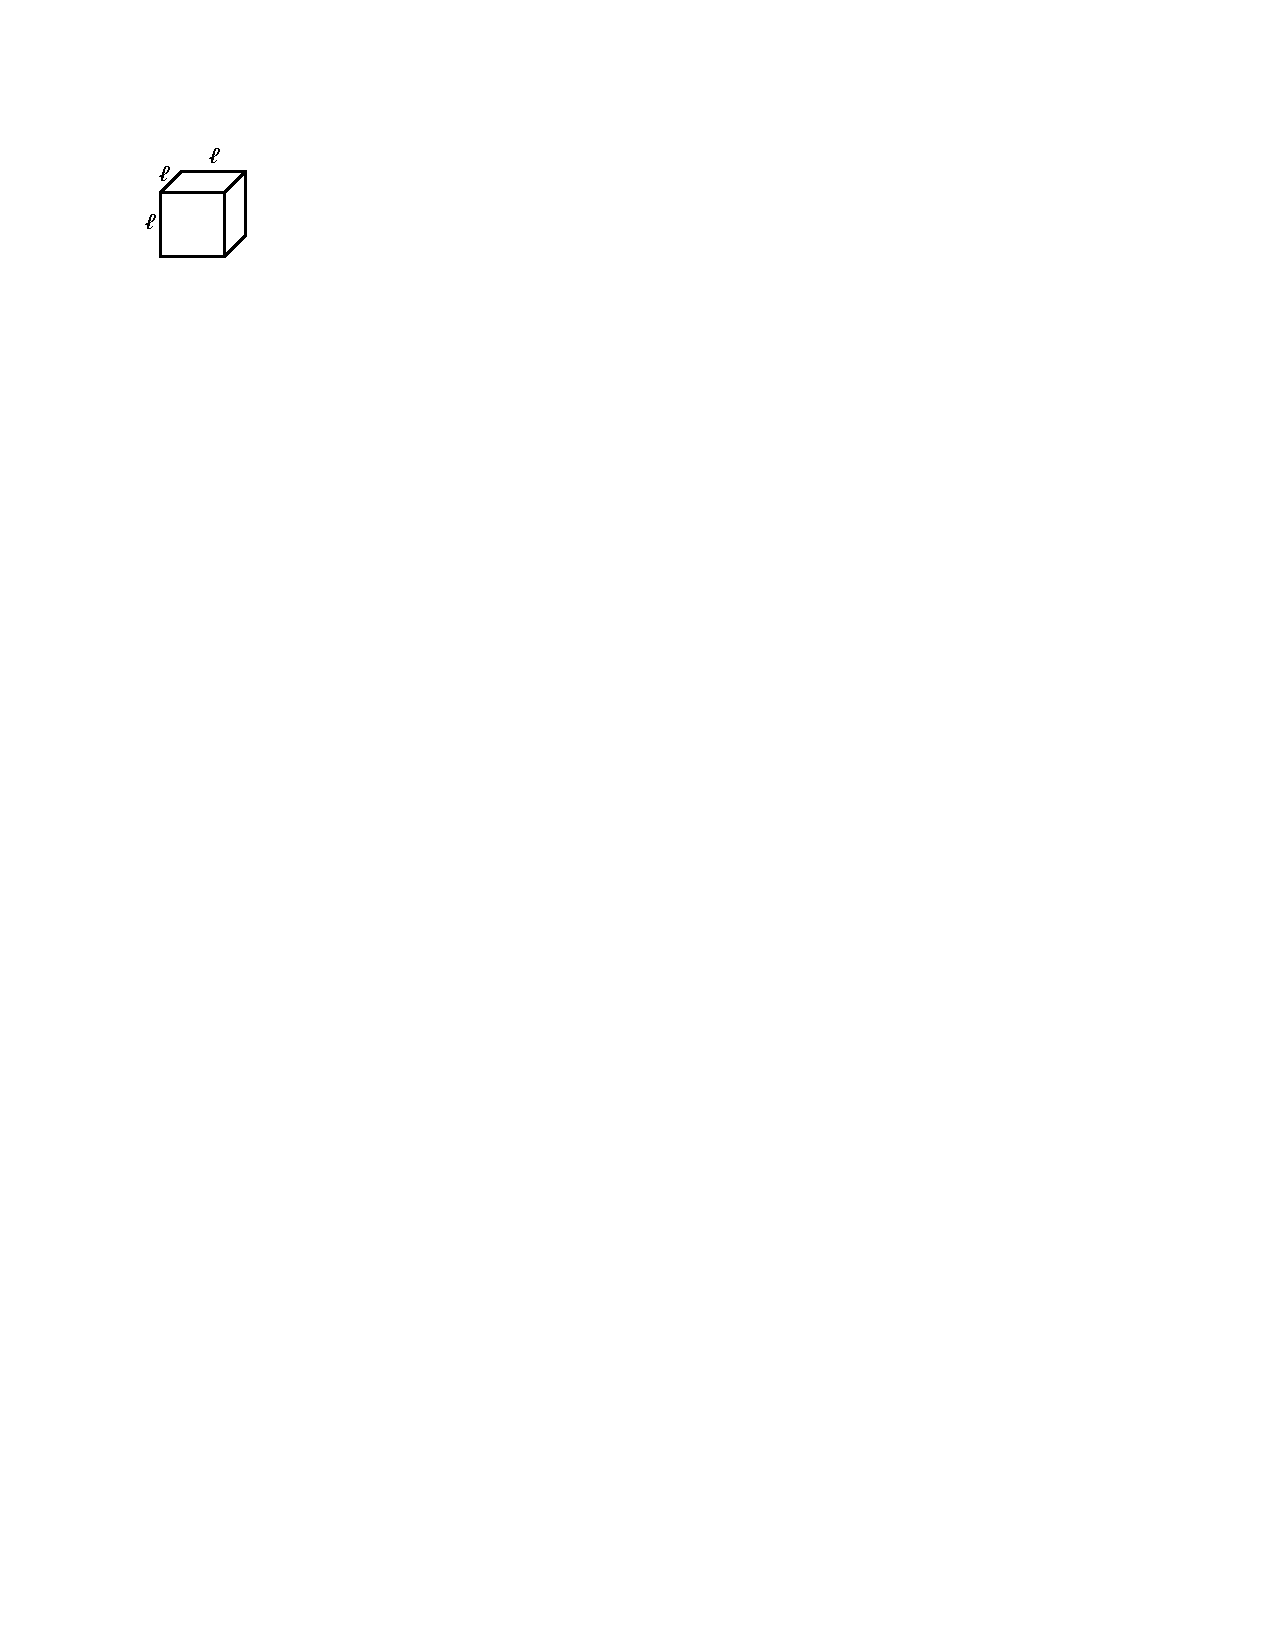
\includegraphics[width=\textwidth]{kin_theory_ideal/box.pdf}
\end{minipage}

%\pagebreak[3]
\item Finally, \textit{pressure} $P$ is defined as the \textit{force per area} acting on the wall.  What exactly is the area of the right-hand wall of this $\ell \times \ell \times \ell$ cube?  And what is its volume $V$?  Use these to write the pressure $P$ on the right-hand wall in terms of only $m$, $v_x$, and $V$.  (Yay!)
\answerspace{0.3in}

\end{enumerate}

\textbf{Activity 2: More Atoms, More Dimensions}

A single atom was a good start, but would make for a sorrowful balloon by itself.  In this part, we'll add more atoms, and think about how they behave on average.


\begin{enumerate}[labparts]

\item First of all, what happens to the pressure on the wall if instead of one single atom, we have $N$ of them?
\answerspace{0.4in}


\item If you looked inside of a balloon with a powerful microscope, would all of the atoms' velocities have the same $x$ component $v_x$?  (Bearing in mind that the correct answer is ``No.'')
\answerspace{0.4in}


No, of course not.  Increasing our number of atoms by $N$ means making the pressure $N$ times larger, but now we need to be careful to write not a specific value of $v_x^2$ for a single atom, but its \textit{average} value over all of the atoms, which we denote here with angle brackets:
$$P=\frac{Nm \left< v_x^2 \right>}{V}.$$

\item The equation above looks kinda awkward with the term $v_x$ still in there.  Let's try to get it just in terms of the speed $v$ instead.  In two dimensions, we can write the speed $v$ of a particle as $v = \sqrt{v_x^2 + v_y^2}$.  Or, if we're thinking about average values, 
$\left< v^2 \right> = \left< v_x^2 \right> + \left< v_y^2 \right> $.
Write the corresponding three-dimensional version of that equation.
\answerspace{0.4in}

\item Now here's the thing: for any \textit{one} atom, $v_x$ and $v_y$ and $v_z$ could all be totally different.  But if we're thinking about \textit{average} values, is there any reason to think that $\left< v_x^2 \right >$ is any different from 
 $\left< v_y^2 \right >$ or $\left< v_z^2 \right >$?
\answerspace{0.4in}

\item Okay, so rewrite your equation for $\left< v^2 \right>$ \textit{only} in terms of $\left< v_x^2 \right>$, and the number ``3''. 
\answerspace{0.4in}

\item Rewrite the equation for $P$ using only $\left< v^2 \right>$ instead of $\left< v_x^2 \right>$.
\answerspace{0.4in}

\end{enumerate}

\pagebreak[3]
\textbf{Activity 3: The Equipartition of Energy}

The equation you wrote above expresses a macroscopic quantity, the pressure $P$, in terms of a microscopic quantity, the average speed $v$.  
$$P=\frac{Nm \left< v^2 \right>}{3V}.$$

In this part, we'll rewrite the expression in terms of only macroscopic quantities.  

\begin{enumerate}[labparts]

\item You remember from Physics 131 that the kinetic energy of a particle is $E_{\rm kin} = \frac{1}{2}mv^2$.  Rewrite the expression for pressure $P$ above in terms of the average kinetic energy of the atoms, $\left<  E_{\rm kin} \right>$.
\answerspace{0.4in}

Here's where we're going to use an extremely powerful idea called the equipartition of energy theorem (or sometimes just the ``equipartition theorem'').  \textit{Equipartition} simply means ``divided equally,'' and the basic idea is that on average, the energy of a system is divided equally among all options.
You saw a taste of equipartition in the previous activity, when you said that on average, $ \left< v_x^2 \right >= \left< v_y^2 \right > = \left< v_z^2 \right > $.  You can think of the kinetic energy of motion along $x$ as 
$\frac{1}{2}mv_x^2$, and the kinetic energy of motion in the other directions as $\frac{1}{2}mv_y^2$ and $\frac{1}{2}mv_z^2$.  On average, these three kinetic energies should all be the same.

Maybe it's obvious that the energies associated with the three directions of translational motion should be the same.  But the equipartition theorem says that the energy is the same for \textit{all} kinds of motion: translational, rotational, and vibrational kinetic energies, and even for potential energies associated with molecular bonds being compressed or stretched.  On average, each possible way that an atom or molecule can move or can store energy, called a ``degree of freedom,'' (DoF) gets the same amount of energy.

Furthermore, the equipartition theorem tells us exactly \textit{how much} energy each degree of freedom gets.  On average, the energy stored in each \textit{mode} or \textit{degree of freedom} is $\frac{1}{2}k_BT$ per particle, where $T$ is the temperature and $k_B$ is Boltzmann's constant, $k_B=1.38 \times 10^{-23}$~J/K.  The total energy for $N$ molecules is given by
$$\textstyle E=N\left(\frac{1}{2}k_BT\right)\bigl({\rm \#DoF}\bigr)$$
where \#DoF is the number of degrees of freedom for each molecule.

\item How many degrees of freedom are there per particle for our system of monatomic gas atoms in the cube?
\answerspace{0.4in}

\item Rewrite your equation for $P$ in terms of $N$, $k_B$, and $T$.  
\answerspace{0.5in}


\item Does your result look familiar to you?  Maybe if you put the $P$ and the $V$ on the same side?
\answerspace{0.5in}

In fact, the expression you've just written is the ideal gas law, $PV = nRT$.  When it's written that way, $n$ is the number of moles, whereas you wrote it with $N$ as the number of individual molecules.  The ``universal gas constant'' $R$ is really just a handy combination of two other constants, 
$$R =k_BN_A=8.31~{\rm J/mol ~K,}$$
where frankly the other two constants are a lot more universal than $R$ is.  ($N_A$ is Avogadro's number, $6.02 \times 10^{23}$ particles/mol, by the way.)

\medskip

Congratulations, you've just learned the equipartition theorem and derived the ideal gas law.  Not bad for a day's work! :-)

\end{enumerate}